% arquivo principal para criar o pdf...
% Não mecher a não ser que saiba o que esta fazendo !!!
% Modificação feita para os alunos de sistemas de informação do IFPR Campus
%Ivaiporã

\documentclass[12pt,openright,oneside,a4paper,main=brazil,english,french,spanish,chapter=TITLE,section=TITLE]{abntex2}
% twoside  use para frente e verso no lugar de oneside 

\usepackage{cmap}
\RequirePackage{ragged2e}	
\usepackage{lmodern}	
\usepackage[T1]{fontenc}
% \usepackage{times}
\usepackage[utf8]{inputenc}		
\usepackage{lastpage}		
\usepackage{indentfirst}
\usepackage{color}	
\usepackage{graphicx}	
\usepackage{units}
% \usepackage[brazilian,hyperpageref]{backref} %serve para contabilizar as citacoes ao final do documento, nas referencias bibliograficas, ver comandos.tex
\usepackage[alf]{abntex2cite}
\usepackage{bold-extra}
\usepackage{eso-pic}
\usepackage{listings} % para codigo-fonte
\usepackage[brazil]{babel}
\usepackage{microtype}
%\usepackage[lmargin=3cm, rmargin=2cm, tmargin=3cm, %bmargin=2cm]{geometry}


% corrige espacamento de paginas pares que ficam diferente das impares
% devido a configuracao de impressao two-side da classe de documento
% remova o setlength abaixo caso queira retorar para a configuracao padrao:
%\setlength{\evensidemargin}{16pt}
\RequirePackage{helvet}
\renewcommand{\familydefault}{\sfdefault}
% ---
% Margens:
% esquerda 3cm direita 2cm
% topo 3cm base 2cm
\setlrmarginsandblock{3cm}{2cm}{*}
\setulmarginsandblock{3cm}{2cm}{*}
\checkandfixthelayout

% O tamanho do parágrafo é dado por:
\setlength{\parindent}{1.3cm}

% Controle do espaçamento entre um parágrafo e outro:
\setlength{\parskip}{0.2cm}  % tente também \onelineskip


\makeevenhead{plain}{}{}{\thepage}
\makeoddhead{plain}{}{}{\thepage}

\makeevenfoot{plain}{}{}{}
\makeoddfoot{plain}{}{}{}
% % caso queira que aparece nas referencias bibliograficas onde tais referencias
% % foram citadas, descomentar tambem o pacote \usepackage[brazilian,hyperpageref]{backref}
% % em pacotes.tex
% \renewcommand{\backrefpagesname}{Citado na(s) página(s):~}
% \renewcommand{\backref}{}
% \renewcommand*{\backrefalt}[4]{
% 	\ifcase #1 %
% 		Nenhuma citação no texto.%
% 	\or
% 		Citado na página #2.%
% 	\else
% 		Citado #1 vezes nas páginas #2.%
% 	\fi}%


\renewcommand{\imprimirdata}{%
    2019
}

\newcommand{\imprimircurso}{Bacharel em Sistemas de Informação}
%\newcommand{\curso}[1]{\def\imprimircurso{#1}}

\newcommand{\palavraChaveUm}[1]{\def\imprimirpalavrachaveum{#1}}
\newcommand{\palavraChaveDois}[1]{\def\imprimirpalavrachavedois{#1}}

\newcommand{\cdu}[1]{\def\nomecdu{#1}}
\newcommand{\dataDaAprovacao}[1]{\def\imprimirdatadaaprovacao{#1}}

\newcommand{\membroConvidadoUm}[1]{\def\imprimirmembroconvidadoum{#1}}
\newcommand{\membroConvidadoDois}[1]{\def\imprimirmembroconvidadodois{#1}}

\newcommand\BackgroundPic{%
	\put(0,0){%
		\parbox[b][\paperheight]{\paperwidth}{%
			\vfill
			\centering
			\includegraphics[width=\paperwidth,height=\paperheight,%
				keepaspectratio]{figuras/ifgformosa2015horizontal01}%
			\vfill
		}
	}
}

%\renewcommand{\imprimircapa}{%
%  \begin{capa}%
%    \center
%	\AddToShipoutPicture*{\BackgroundPic}
%
%%	\begin{huge}
%%		\textbf{\textsc{Trabalho de Conclusão de Curso}}
%%	\end{huge}
%
%    \vspace*{2.7in}
%	{\textbf{\large\imprimirinstituicao}}
%	\par
%	{\textbf{\large\imprimircurso}}
%
%	\vspace{0.5in}
%
%    {\ABNTEXchapterfont\bfseries\LARGE\imprimirtitulo}
%    \vspace*{\fill}
%    
%	\begin{flushright}
%    	\textbf{{\large{Autor: \imprimirautor}}}
%		\par
%    	\textbf{{\large{Orientador: \imprimirorientador}}}
%	\end{flushright}
%		
%    \vspace*{0.2in}
%    \textbf{{\large\imprimirlocal}}
%    \par
%    \textbf{{\large\imprimirdata}}
%    
%    \vspace*{2.2in}
%  \end{capa}
%}

\renewcommand{\imprimircapa}{%
	\begin{capa}%
		
		\vspace*{-2.2cm}
		\hspace*{-1cm}
		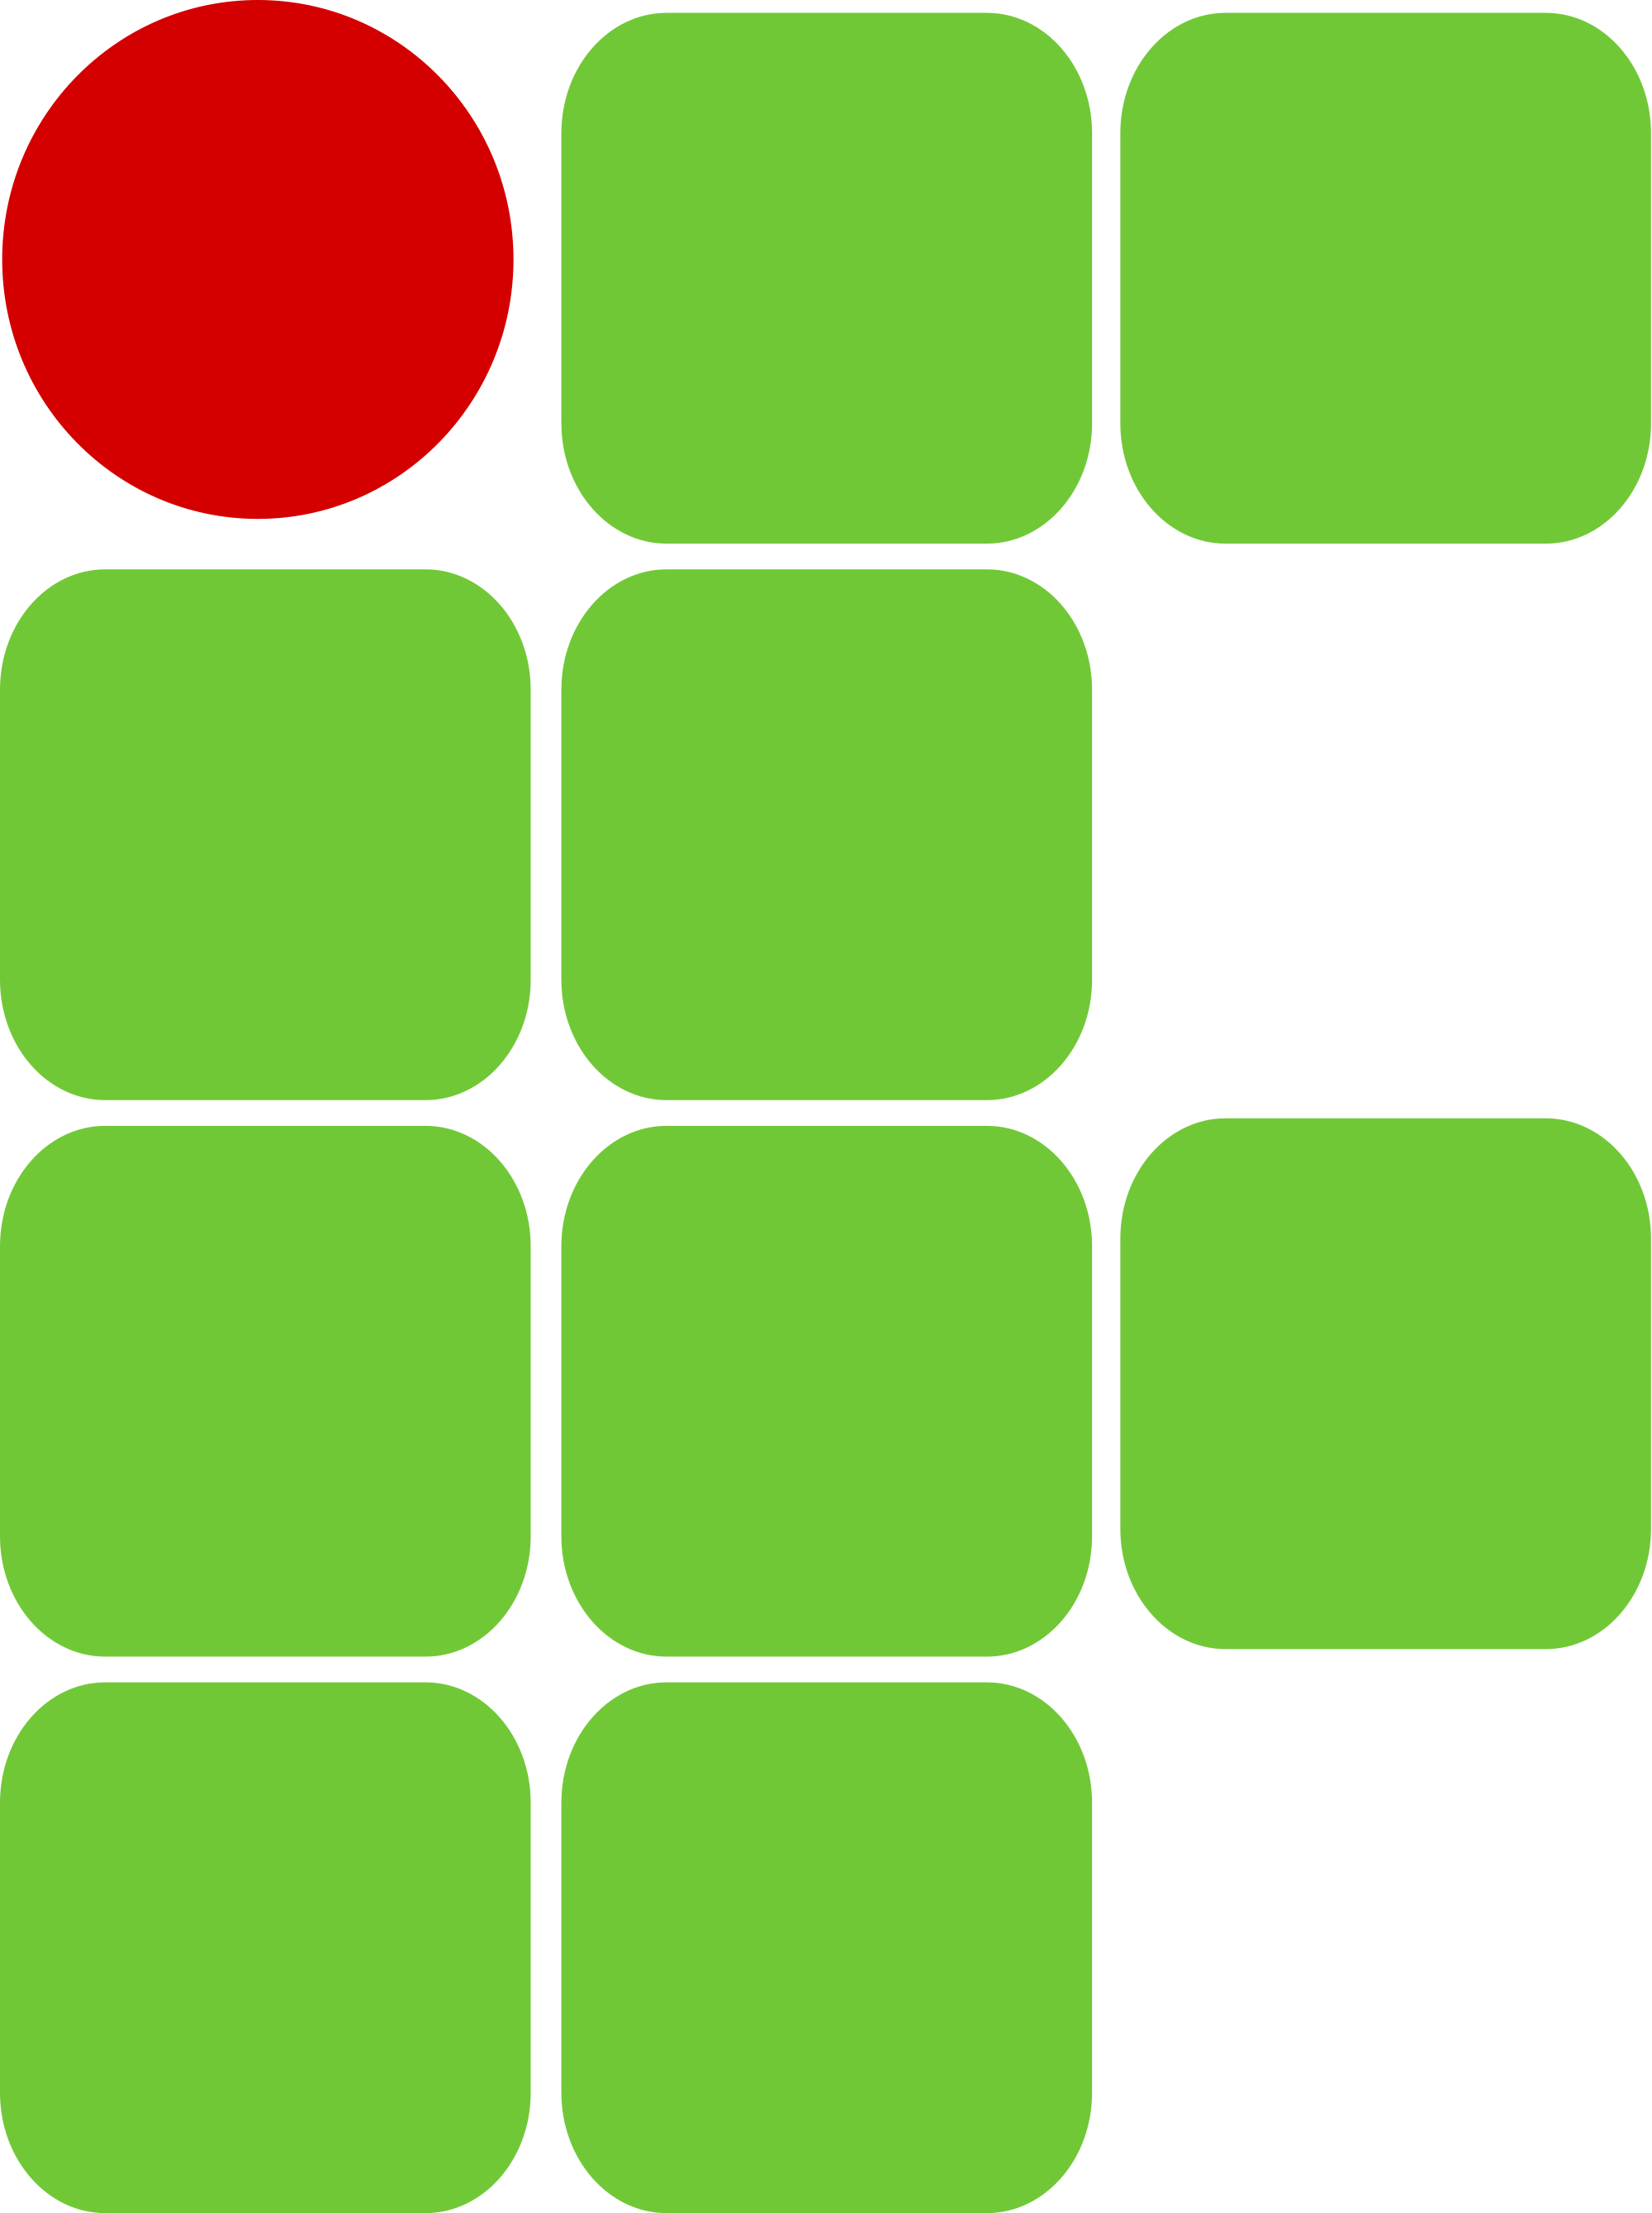
\includegraphics[width=1.5cm]{imagens/logo.png}
		\center
		\large INSTITUTO FEDERAL DO PARANÁ
		
		\vspace*{1cm}
		
		\MakeUppercase{\large\imprimirautor}
		
		\vfill
		\begin{center}
			\MakeUppercase{\large\bfseries\imprimirtitulo}
		\end{center}
		\vfill
		
		\MakeUppercase{\large\imprimirlocal}
		
		\large\imprimirdata
		
		\vspace*{1cm}
	\end{capa}
}

% os itens abaixo configuram a exibicao da lista de algoritmos
\renewcommand\lstlistingname{Algoritmo}
\renewcommand\lstlistlistingname{Lista de Algoritmos}
\let\oldlstlistoflistings\lstlistoflistings
\renewcommand{\lstlistoflistings}{%
  \begingroup%
  \let\oldnumberline\numberline%
  \renewcommand{\numberline}{\lstlistingname~\oldnumberline}%
  \oldlstlistoflistings%
  \endgroup}

% Configuração de fontes
\renewcommand{\ABNTEXchapterfont}{\bfseries}
\renewcommand{\ABNTEXchapterfontsize}{\normalsize}

\renewcommand{\ABNTEXpartfont}{\ABNTEXchapterfont}
\renewcommand{\ABNTEXpartfontsize}{\normalsize}

\renewcommand{\ABNTEXsectionfont}{\ABNTEXchapterfont}
\renewcommand{\ABNTEXsectionfontsize}{\normalsize}

\renewcommand{\ABNTEXsubsectionfont}{\sffamily}
\renewcommand{\ABNTEXsubsectionfontsize}{\normalsize}

\renewcommand{\ABNTEXsubsubsectionfont}{\sffamily}
\renewcommand{\ABNTEXsubsubsectionfontsize}{\normalsize}

\renewcommand{\ABNTEXsubsubsubsectionfont}{\sffamily}
\renewcommand{\ABNTEXsubsubsubsectionfontsize}{\normalsize}

% Dados pessoais
\autor{Richardson Schawarski}


% Dados do trabalho
\titulo{Free BSD}
\data{2019}
\palavraChaveUm{Unix}
\palavraChaveDois{BSD}

% Dados da orientacao
\orientador{NEYLOR GARCIA BACHIEGA}
%\coorientador{(quando houver, Titulação Acadêmica e Nome do Orientador)}

% Dados para a ficha catalográfica
\cdu{02:141:005.6}

% Dados da aprovação do trabalho
\dataDaAprovacao{01 de junho de 2016}
\membroConvidadoUm{Titulação e Nome do Professor Convidado 01}
\membroConvidadoDois{Titulação e Nome do Professor Convidado 02}

\local{Ivaiporã, PR}

\tipotrabalho{Trabalho de Conclusão de Curso}
\preambulo{Monografia submetida ao curso de graduação em  \imprimircurso{}
 	Instituto Federal do Paraná  , Ivaiporã Camaquã, como requisito parcial para obtenção do Título 
de Bacharel em Sistemas de Informação}

\definecolor{blue}{RGB}{41,5,195}
\makeatletter
\hypersetup{
     	%pagebackref=true,
		pdftitle={\@title}, 
		pdfauthor={\@author},
    	pdfsubject={\imprimirpreambulo},
	    pdfcreator={LaTeX with abnTeX2},
		pdfkeywords={abnt}{latex}{abntex}{abntex2}{trabalho acadêmico}, 
		colorlinks=true,       		% false: boxed links; true: colored links
    	linkcolor=blue,          	% color of internal links
    	citecolor=blue,        		% color of links to bibliography
    	filecolor=magenta,      		% color of file links
		urlcolor=blue,
		bookmarksdepth=4
}
\makeatother
\setlength{\parindent}{1.3cm}
\setlength{\parskip}{0.2cm}  
\makeindex



% configuracao de exibicao de codigo-fonte
\definecolor{dkgreen}{rgb}{0,0.6,0}
\definecolor{gray}{rgb}{0.5,0.5,0.5}
\definecolor{mauve}{rgb}{0.58,0,0.82}

\lstset{frame=tb,
  language=Java,
  aboveskip=3mm,
  belowskip=3mm,
  showstringspaces=false,
  columns=flexible,
  basicstyle={\small\ttfamily},
  numbers=left,
  numberstyle=\tiny\color{gray},
  keywordstyle=\color{blue},
  commentstyle=\color{dkgreen},
  stringstyle=\color{mauve},
  breaklines=true,
  breakatwhitespace=true,
  tabsize=4,
  xleftmargin=0.6cm,
  numberbychapter=false % se true, enumera os algoritmos com o capitulo (Algoritmo 3.1) %
%   frame=single, % se for necessario cricao de um quadro (frame)
%   framexleftmargin=1.5em % se for necessario cricao de um quadro (frame)
}



\begin{document}
	
	\frenchspacing 
	\imprimircapa
	\imprimirfolhaderosto*
	
	\begin{fichacatalografica}
	\vspace*{\fill}					% Posição vertical
	\hrule							% Linha horizontal
	\begin{center}					% Minipage Centralizado
	\begin{minipage}[c]{12.5cm}		% Largura
	
	\imprimirautor
	
	\hspace{0.5cm} \imprimirtitulo  / \imprimirautor. --
	\imprimirlocal, \imprimirdata-
	
	\hspace{0.5cm} \pageref{LastPage} p. : il. (algumas color.) ; 30 cm.\\
	
	\hspace{0.5cm} \imprimirorientadorRotulo~\imprimirorientador\\
	
	\hspace{0.5cm}
	\parbox[t]{\textwidth}{\imprimirtipotrabalho~--~\imprimirinstituicao,
	\imprimirdata.}\\
	
	\hspace{0.5cm}
		1. \imprimirpalavrachaveum.
		2. \imprimirpalavrachavedois.
		I. \imprimirorientador.
		II.Instituto Federal Paraná.
		III. Câmpus Ivaiporã.
		IV. \imprimirtitulo\\ 			
	
	\hspace{8.75cm} CDU \nomecdu\\
	
	\end{minipage}
	\end{center}
	\hrule
\end{fichacatalografica}

	% \begin{errata}
Elemento opcional da \citeonline[4.2.1.2]{NBR14724:2011}. \textbf{Caso não 
deseje uma errata, deixar todo este arquivo em branco}. Exemplo:

\vspace{\onelineskip}

FERRIGNO, C. R. A. \textbf{Tratamento de neoplasias ósseas apendiculares com
reimplantação de enxerto ósseo autólogo autoclavado associado ao plasma
rico em plaquetas}: estudo crítico na cirurgia de preservação de membro em
cães. 2011. 128 f. Tese (Livre-Docência) - Faculdade de Medicina Veterinária e
Zootecnia, Universidade de São Paulo, São Paulo, 2011.

\begin{table}[htb]
\center
\footnotesize
\begin{tabular}{|p{1.4cm}|p{1cm}|p{3cm}|p{3cm}|}
  \hline
   \textbf{Folha} & \textbf{Linha}  & \textbf{Onde se lê}  & \textbf{Leia-se}  \\
    \hline
    1 & 10 & auto-conclavo & autoconclavo\\
   \hline
\end{tabular}
\end{table}

\end{errata}

%\begin{folhadeaprovacao}
	\begin{center}
		\begin{center}
			\ABNTEXchapterfont\bfseries FOLHA DE APROVAÇÃO
			\par
			\vspace*{1.5cm}
			{\normalfont\ABNTEXchapterfontsize\MakeUppercase\imprimirautor}
			\vspace*{1.5cm}
			\par
			{\normalfont\ABNTEXchapterfontsize\MakeUppercase\imprimirtitulo}
		\end{center}
		\vspace*{\fill}
		
		\hspace{.45\textwidth}
		\begin{minipage}{.5\textwidth}
			\imprimirpreambulo
		\end{minipage}%
		\vspace*{\fill}
	\end{center}
	
   	\assinatura{\textbf{\imprimirorientador} \\ Orientador} 
	\assinatura{\textbf{diretor} \\ Convidado 1}
	\assinatura{\textbf{diretor2} \\ Convidado 2}
	%\assinatura{\textbf{Professor} \\ Convidado 3}
	%\assinatura{\textbf{Professor} \\ Convidado 4}
	
	\vspace{3cm}
	\begin{center}
		\imprimirlocal, 10 de novembro de 2000.
	\end{center}
	
	\pagebreak
\end{folhadeaprovacao}



%	\begin{dedicatoria}
   \vspace*{21cm}
   \centering
   \noindent
	\textbf{A dedicatória é opcional. Caso não deseje uma, remova esta página}.

   \textit{Este trabalho é dedicado às crianças adultas que,\\
   quando pequenas, sonharam em se tornar cientistas.} \vspace*{\fill}

\end{dedicatoria}

	\begin{agradecimentos}
A inclusão desta seção de agradecimentos é opcional, portanto, sua inclusão 
fica a critério do(s) autor(es), que caso deseje(em) fazê-lo deverá(ão) 
utilizar este espaço, seguindo a formatação de \textit{espaço simples e 
fonte padrão do texto (arial ou times, tamanho 12 sem negritos, aspas ou 
itálico}.

\textbf{Caso não deseje utilizar os agradecimentos, remova esta página}.
\end{agradecimentos}

	\begin{epigrafe}
    \vspace*{\fill}
	\begin{flushright}
	
		
		\textit{``Os que se encantam com a prática sem a ciência são \\
		como os timoneiros que entram no navio sem timão\\
		nem bússola, nunca tendo certeza do seu destino". \\
		(Leonardo da Vinci)}
	\end{flushright}
\end{epigrafe}

	\begin{resumo}
 O resumo deve ressaltar o objetivo, o método, os resultados e as conclusões 
 do documento. A ordem e a extensão
 destes itens dependem do tipo de resumo (informativo ou indicativo) e do
 tratamento que cada item recebe no documento original. O resumo deve ser
 precedido da referência do documento, com exceção do resumo inserido no
 próprio documento. (\ldots) As palavras-chave devem figurar logo abaixo do
 resumo, antecedidas da expressão Palavras-chave:, separadas entre si por
 ponto e finalizadas também por ponto. O texto pode conter no mínimo 150 e 
 no máximo 500 palavras, é aconselhável que sejam utilizadas 200 palavras. 
 E não se separa o texto do resumo em parágrafos.

 \vspace{\onelineskip}
    
 \noindent
 \textbf{Palavras-chaves}: latex. abntex. editoração de texto.
\end{resumo}

	\begin{resumo}[Abstract]
 \begin{otherlanguage*}{english}
  Silvio Santos Ipsum mah você mora com o papai ou com a mamãem? O Raul Gil é gayam! ... Maa O Ah Ae! Ih Ih! O Raul Gil é gayamm! Wellintaaammmmmmmmm. No duro? É com você Lombardiam. Mah roda a roduamm. Ma tem ou no tem o celular do milhãouamm? Vem pra lá, mah você vai pra cá. Agora vai, agora vem pra lamm. Eu não queria perguntar isso publicamenteam, ma vou perguntar. Carla, você tem o ensino fundamentauam? Mah você não consegue né Moisés? Você não consegueam. No duro? É por sua conta e riscoamm? Ha haeeee. Hi hi. Ma tem ou no tem o celular do milhãouamm? Mah você não consegue né Moisés? Você não consegueam. Ma vai pra lá. Ma voc está certo dissoam? Mah você mora com o papai ou com a mamãem? Ma vale dérreaisam? Ha haeeee. Hi hi. Ma vale dérreaisam? Você veio da.

   \vspace{\onelineskip}
 
   \noindent 
   \textbf{Key-words}: latex. abntex. text editoration.
 \end{otherlanguage*}
\end{resumo}

	% geracao dos sumario sde listas (figuras, tabelas, algoritmos, etc.)
\pdfbookmark[0]{\listfigurename}{lof}
\listoffigures*
\cleardoublepage
\pdfbookmark[0]{\listtablename}{lot}
\listoftables*
\cleardoublepage
\pdfbookmark[0]{\lstlistlistingname}{lol}
\begin{KeepFromToc} %remove lista de algoritmos do sumario
\lstlistoflistings %lista de algoritmos aqui
\end{KeepFromToc}
\cleardoublepage

	\begin{siglas}
  \item[Fig.] Area of the $i^{th}$ component
  \item[456] Isto é um número
  \item[123] Isto é outro número
  \item[lauro cesar] este é o meu nome
\end{siglas}

	\begin{simbolos}
  \item[$ \Gamma $] Letra grega Gama
  \item[$ \Lambda $] Lambda
  \item[$ \zeta $] Letra grega minúscula zeta
  \item[$ \in $] Pertence
\end{simbolos}

	\pdfbookmark[0]{\contentsname}{toc}
\tableofcontents*
\cleardoublepage

	
	\textual
	
	%\chapter*[Aviso Geral]{Aviso Geral}
\addcontentsline{toc}{chapter}{Aviso Geral} %adicionar ao sumario para contar pagina


Estas instruções apresentam um conjunto mínimo de exigências necessárias a 
uniformidade de apresentação do relatório de Trabalho de Conclusão de Curso de Tecnologia em Análise e Desenvolvimento de Sistemas no câmpus Camaquã (IFSUL). O presente documento é uma versão baseada do documento de TCC do Instituto Federal de Goiás câmpus Formosa\footnote{\url{https://pt.overleaf.com/latex/templates/template-para-tcc-do-curso-tads-no-ifg-formosa/pvbdgztbmnbh}}. Nesta versão, utilizou-se os textos fornecidos pela versão do câmpus de Formosa com a adição de textos próprios. Seções foram alteradas, removidas e resumidas, a fim de refletir as necessidades do curso. Vários comandos e pacotes foram refatorados devido a sua integralização com a plataforma Overleaf e com adições específicas de estruturas, como a formatação de algoritmos, por exemplo (inexistente na versão base).

Estilo, concisão e clareza ficam inteiramente sob a responsabilidade do(s) aluno(s) autor(es) do relatório. Para outras instituições e/ou cursos, o uso e edição deste \textit{template} é completamente livre, mantendo as diretrizes conforme licença designada nesta versão.


\textbf{Remova esta página antes de entregar este documento.}


	\chapter[Introdução]{\uppercase{Introdução}}


A regra mais rígida com respeito a Introdução é que a mesma, que é 
necessariamente parte integrante do texto, não deverá fazer agradecimentos 
a pessoas ou instituições nem comentários pessoais do autor atinentes à 
escolha ou à relevância do tema.

A Introdução obedece a critérios do Método Cientifico e a exigências 
didáticas. Na Introdução o leitor deve ser colocado dentro do espírito do 
trabalho.

Cabe mencionar que a Introdução de um trabalho pode, pelo menos em parte, 
ser escrita com grande vantagem uma vez concluído o trabalho (ou o 
Desenvolvimento e as Conclusões terem sido redigidos). Não só a pesquisa 
costuma modificar-se durante a execução, mas também, ao fim do trabalho, o 
autor tem melhor perspectiva ou visão de conjunto.

Por seu caráter didático, a Introdução deve, ao seu primeiro parágrafo, 
sugerir o mais claramente possível o que pretende o autor. Em seguida deve 
procurar situar o problema a ser examinado em relação ao desenvolvimento 
científico e técnico do momento. Assim sendo, sempre que pertinente, os 
seguintes pontos devem ser abordados: \citeonline{richardson}

\begin{itemize}

	\item Contextualização ou apresentação do tema em linhas gerais de 
	forma clara e objetiva;
	\item Apresentação da justificativa e/ou relevância do tema escolhido;
	\item Apresentação da questão ou problema de pesquisa;
	\item Declaração dos objetivos, gerais e específicos do trabalho;
	\item Apresentação da metodologia, e
	\item Indicação de como o trabalho estará organizado.

\end{itemize}

\section{Objetivos}

Especificação do objetivo geral do trabalho, definido em um parágrafo.

\subsection{Objetivos Específicos}

Os objetivos específicos devem ser listados aqui, é recomendado que seja fornecida através de uma lista.

\section{Metodologia}

Metodologia é a descrição de todos os passos metodológicos utilizados no trabalho. Sugere-se que se enfatize especialmente em (1) População ou Sujeitos da pesquisa, (2) Materiais e equipamentos utilizados e (3) Procedimentos de coleta de dados. 

Para cada objetivo específico recomenda-se um ou mais parágrafos descrevendo as atividades necessárias para a sua resolução. Informe, por exemplo, pesquisas a serem realizadas, dados a serem coletados, tecnologias a serem estudas e aplicadas.

\subsection{Estrutura do Trabalho}

A formatação do trabalho como um todo considera três elementos principais: 
(1) pré-textuais, (2) textuais e (3) pós-textuais. Cada um destes, pode se 
subdividir em outros elementos formando a estrutura global do trabalho, 
conforme abaixo (as entradas itálico são \textit{opcionais}; em itálico e
negrito são \textbf{\textit{essenciais}}):

\begin{description}
	\item [Pré-textuais] \

	\begin{itemize}
		\item Capa
		\item Folha de rosto
		\item \textit{Dedicatória}
		\item \textit{Agradecimentos}
		\item \textit{Epígrafe}
		\item Resumo
		\item Abstract
		\item Lista de figuras
		\item Lista de tabelas
		\item Lista de símbolos e
		\item Sumário
	\end{itemize}

	\item [Textuais] \

	\begin{itemize}
		\item \textbf{\textit{Introdução}}
		\item \textbf{\textit{Desenvolvimento}}
		\item \textbf{\textit{Conclusões}}
	\end{itemize}

	\item [Pós-Textuais] \
	
	\begin{itemize}
		\item Referências bibliográficas
		\item \textit{Bibliografia}
		\item Anexos
		\item Contracapa
	\end{itemize}
\end{description}

Os aspectos específicos da formatação de cada uma dessas três partes 
principais do relatório são tratados nos capítulos e seções seguintes.

No modelo \LaTeX, os arquivos correspondentes a estas estruturas que devem
ser editados manualmente estão na pasta \textbf{editáveis}. Os arquivos
da pasta \textbf{fixos} tratam os elementos que não necessitam de 
edição direta, e devem ser deixados como estão na grande maioria dos casos.

\section{Considerações sobre formatação básica do relatório}

A seguir são apresentadas as orientações básicas sobre a formatação do
documento. O modelo \LaTeX\ já configura todas estas opções corretamente,
de modo que para os usuários deste modelo o texto a seguir é meramente
informativo.

\subsection{Tipo de papel, fonte e margens}

Papel - Na confecção do relatório deverá ser empregado papel branco no 
formato padrão A4 (21 cm x 29,7cm), com 75 a 90 g/m2.

Fonte – Deve-se utilizar as fontes Arial ou Times New Roman no tamanho 12 
pra corpo do texto, com variações para tamanho 10 permitidas para a 
paginação, legendas e notas de rodapé. Em citações diretas de mais de três 
linhas utilizar a fonte tamanho 10, sem itálicos, negritos ou aspas. Os 
tipos itálicos são usados para nomes científicos e expressões estrangeiras, 
exceto expressões latinas.

Margens - As margens delimitando a região na qual todo o texto deverá estar 
contido serão as seguintes: 

\begin{itemize}
	\item Esquerda: 03 cm;
	\item Direita	: 02 cm;
	\item Superior: 03 cm;
	\item Inferior: 02 cm. 
\end{itemize}

\subsubsection{Numeração de Páginas}

A contagem sequencial para a numeração de páginas começa a partir da 
primeira folha do trabalho que é a Folha de Rosto, contudo a numeração em 
si só deve ser iniciada a partir da primeira folha dos elementos textuais. 
Assim, as páginas dos elementos pré-textuais contam, mas não são numeradas 
e os números de página aparecem a partir da primeira folha dos elementos 
textuais que é a Introdução. 

Os números devem estar em algarismos arábicos (fonte Times ou Arial 10) no 
canto superior direito da folha, a 02 cm da borda superior, sem traços, 
pontos ou parênteses. 

A paginação de Apêndices e Anexos deve ser contínua, dando seguimento ao 
texto principal.

\subsubsection{Espaços e alinhamento}

Para a monografia de TCC o espaço entrelinhas do corpo do texto 
deve ser de 1,5 cm, exceto RESUMO, CITAÇÔES de mais de três linhas, NOTAS 
de rodapé, LEGENDAS e REFERÊNCIAS que devem possuir espaçamento simples. 
Ainda, ao se iniciar a primeira linha de cada novo parágrafo se deve 
tabular a distância de 1,25 cm da margem esquerda.

Quanto aos títulos das seções primárias da monografia, estes devem começar 
na parte superior da folha e separados do texto que o sucede, por um espaço 
de 1,5 cm entrelinhas, assim como os títulos das seções secundárias, 
terciárias. 

A formatação de alinhamento deve ser justificado, de modo que o texto fique 
alinhado uniformemente ao longo das margens esquerda e direita, exceto para 
CITAÇÕES de mais de três linhas que devem ser alinhadas a 04 cm da margem 
esquerda e REFERÊNCIAS que são alinhadas somente à margem esquerda do texto 
diferenciando cada referência.

\subsubsection{Quebra de Capítulos e Aproveitamento de Páginas}

Cada seção ou capítulo deverá começar numa nova pagina (recomenda-se que 
para texto muito longos o autor divida seu documento em mais de um arquivo 
eletrônico). 

Caso a última pagina de um capitulo tenha apenas um número reduzido de 
linhas (digamos 2 ou 3), verificar a possibilidade de modificar o texto 
(sem prejuízo do conteúdo e obedecendo as normas aqui colocadas) para 
evitar a ocorrência de uma página pouco aproveitada.

Ainda com respeito ao preenchimento das páginas, este deve ser otimizado, 
evitando-se espaços vazios desnecessários. 

Caso as dimensões de uma figura ou tabela impeçam que a mesma seja 
posicionada ao final de uma página, o deslocamento para a página seguinte 
não deve acarretar um vazio na pagina anterior. Para evitar tal ocorrência, 
deve-se re-posicionar os blocos de texto para o preenchimento de vazios. 

Tabelas e figuras devem, sempre que possível, utilizar o espaço disponível 
da página evitando-se a \lq\lq quebra\rq\rq\ da figura ou tabela. 

	\chapter[Fundamentação Teórica]{Fundamentação Teórica}

Referencial teórico, que corresponde a uma análise dos trabalhos relevantes, encontrados na pesquisa bibliográfica sobre o assunto. Este capítulo é a primeira parte do Corpo do Trabalho e pode ser subdividido em seções de acordo com o planejamento do autor. As seções primárias são aquelas que  resultam da primeira divisão do texto do documento, geralmente correspondendo a divisão em capítulos. Seções secundárias, terciárias, etc., são aquelas que resultam da divisão do texto de uma seção primária, secundária, terciária, etc., respectivamente.

As seções primárias são numeradas consecutivamente, seguindo a série natural de números inteiros, a partir de 1, pela ordem de sua sucessão no 
documento.


\section{Uso de editores de texto}

O uso de programas de edição eletrônica de textos é de livre escolha do autor. 


	
\chapter[Desenvolvimento]{Desenvolvimento}

O Desenvolvimento (segunda parte do Corpo do Trabalho) é subdividido em seções de acordo com o planejamento do autor. É exigido organização, objetividade e clareza. É conveniente dividi-lo nas seguintes partes:

\begin{itemize}

	\item Projeto, requisitos e outras definições sobre o problema a ser resolvido, identificado em seções anteriores.
	\item Implementação do projeto, discussões sobre codificação (se aplicado ao tema).
	\item Avaliação, testes ou outras análises sobre o projeto, direcionando o leitor para as conclusões do projeto.

\end{itemize}



\section{Corpo do Texto}

O estilo de redação deve atentar a boa prática da linguagem técnica. Para a terminologia metrological usar o Vocabulário Internacional de Termos Fundamentais e Gerais de Metrologia \cite{inmetro2003}  (Instituto Nacional de Metrologia, 2003).

Grandezas dimensionais devem ser apresentadas em unidades consistentes com  o Sistema Internacional de Unidades  (SI). Outras unidades podem ser usadas  como unidades secundárias entre parenteses se necessário. Exceções são relacionadas a unidades não-SI usadas como identificadores comerciais como pro exemplo \lq\lq disquete de  3$\nicefrac{1}{2}$ polegadas\rq\rq. 

Na apresentação de números ao longo do texto usar virgula para separar a parte decimal de um número. Resultados experimentais devem ser apresentados com sua respectiva incerteza de medição.

\section{Títulos de capítulos e seções}

Recomendações de formatação de seções. 

\begin{description}

	\item 1 SEÇÃO PRIMÁRIA - MAIÚSCULAS; normal; tamanho 16;

	\item 1.1 Seção Secundária - Minúsculas, com exceção da primeira letra; normal; tamanho 14;

	\item 1.1.1 Seção terciária - Minúsculas, com exceção da 
	primeira letra; normal; tamanho 12;

	\item Os demais níveis seguem formatação do nível acima. 

\end{description}



\section{Notas de rodapé}

Notas eventualmente necessárias devem ser numeradas de forma sequencial ao longo do texto no formato 1, 2, 3... sendo posicionadas no rodapé de cada página na qual a nota é utilizada.\footnote{Como, por exemplo, esta nota}.

\section{Legendas}

As legendas devem ser numeradas sequencialmente e agrupadas sobre um conjunto. Os grupos de legendas são, por exemplo, os de Figuras, Equações, Quadros, Tabelas e Algoritmos. O número sequencial pode fazer relação com a seção mas isto não é obrigatório. As seções a seguir descrevem detalhes sobre estes conjuntos.

\section{Equações}

Equações matemáticas devem ser numeradas sequencialmente e alinhadas a esquerda com recuo de 0,6 cm. Usar numerais arábicos entre parênteses, alinhado a direita, no formato Times New Roman de 9 pts. para numerara as equações como mostrado na Eq. (\ref{eqn01}).

Referências a equações no corpo do texto devem ser feitas como \lq\lq Eq. (\ref{eqn01})\rq\rq\ quando no meio de uma frase ou como \lq\lq Equação (\ref{eqn01})\rq\rq\ quando no inicio de uma sentença. Um espaçamento de 11 pontos deve ser deixado acima, abaixo e entre equações subsequentes. Para uma apresentação compacta das equações deve-se usar os símbolos e expressões matemáticas mais adequados e parênteses para evitar ambiguidades em denominadores. Os símbolos usados nas equações citados no texto devem apresentar exatamente a mesma formatação usada nas equações.
\begin{equation}
\label{eqn01}
	\frac{d\mathbf{C}}{dw} = \frac{du}{dw}\cdot \mathbf{F}_u + 
		\frac{dv}{dw}\cdot \mathbf{F}_v 
\end{equation}

O significado de todos os símbolos mostrados nas equações deve ser apresentado na lista de símbolos no inicio do trabalho, embora, em certas circunstancias o autor possa para maior clareza descrever o significado de certos símbolos no corpo do texto, logo após a equação.


\section{Figuras e Gráficos}

As figuras devem ser centradas entre margens e identificadas por uma legenda alinhada a esquerda com recuo especial de deslocamento de 1,8 cm, com mostrado 
na Fig. (\ref{fig01}). O tamanho das fontes empregadas nos rótulos e anotações 
usadas nas figuras deve ser compatível com o usado no corpo do texto. Rótulos e 
anotações devem estar em português, com todas as grandezas mostradas em 
unidades do SI (Sistema Internacional de unidades).

Todas as figuras, gráficos e fotografias devem ser numeradas e referidas no 
corpo do texto adotando uma numeração sequencial de identificação. As figuras e 
gráficos devem ser claras e com qualidade adequada para eventual reprodução 
posterior tanto em cores quanto em preto-e-branco.


As abscissas e ordenadas de todos os gráficos devem ser rotuladas com seus 
respectivos títulos em português seguida da unidade no SI que caracteriza a 
grandes entre colchetes. 

\begin{figure}[hbt!]
	\centering
		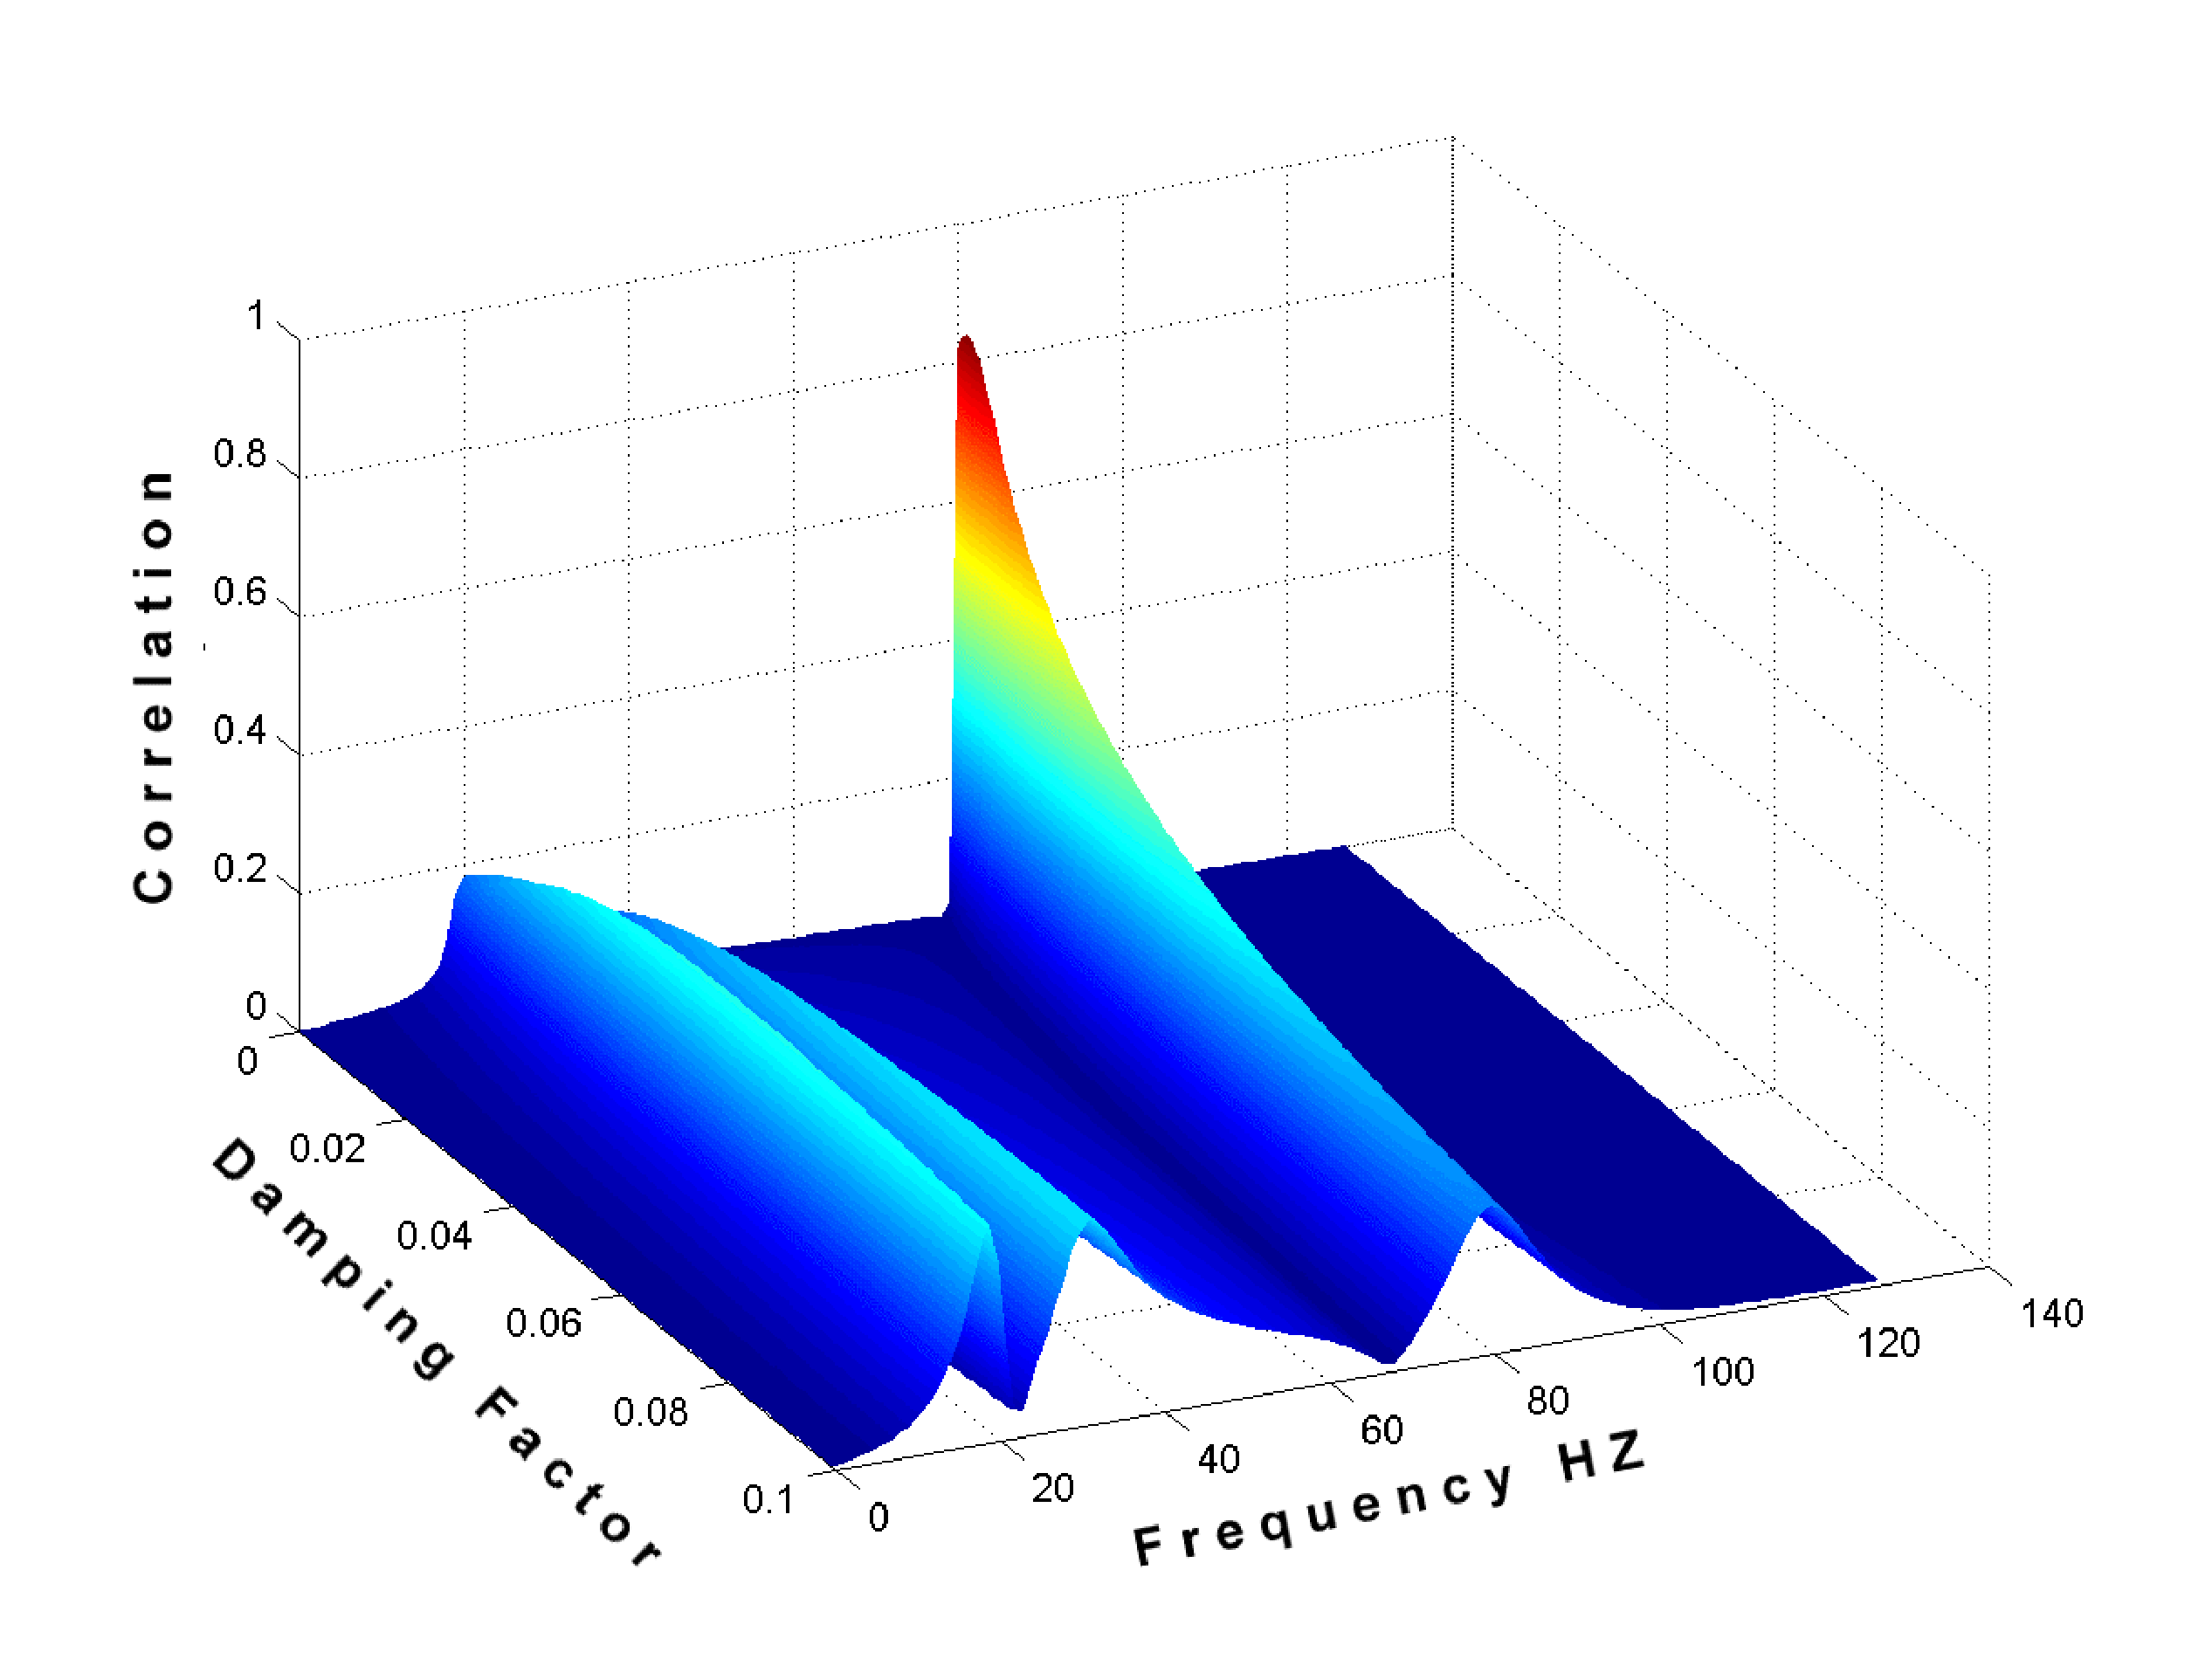
\includegraphics[keepaspectratio=true,scale=0.3]{imagens/fig01.eps}
	\caption{Correlação de coeficientes Wavelets.}
	\label{fig01}
\end{figure}


A referência explícita no texto à uma figura deve ser feita como 
\lq\lq Fig. (\ref{fig01})\rq\rq\ quando no meio de uma frase ou como 
\lq\lq Figura (\ref{fig01})\rq\rq\ quando no início da mesma. Referencias 
implícitas a uma dada figura devem ser feitas entre parênteses como 
(Fig. \ref{fig01}). Para referências a mais de uma figura as mesmas regras 
devem ser aplicadas usando-se o plural adequadamente. Exemplos:

\begin{itemize}
	\item \lq\lq Após os ensaios experimentais, foram obtidos os resultados 
	mostrados na Fig. (\ref{fig01}), que ...\rq\rq
	\item \lq\lq A Figura (\ref{fig01}) apresenta os resultados obtidos, onde 
	pode-se observar que ...\rq\rq
	\item \lq\lq As Figuras (1) a (3) apresentam os resultados obtidos, 
	...\rq\rq
	\item \lq\lq Verificou-se uma forte dependência entre as variáveis citadas 
	(Fig. \ref{fig01}), comprovando ...\rq\rq
\end{itemize}

É recomendado (não obrigatório) que cada figura deve ser posicionada o mais próxima possível da primeira citação feita à mesma no texto, imediatamente após o parágrafo no qual é feita tal citação, se possível, na mesma página.


\section{Tabela}

As tabelas devem estar centradas entre margens e identificadas por uma legenda alinhada a esquerda, com recuo especial de deslocamento de 1,8 cm, posicionada acima da tabela com mostrado nas Tabs. (\ref{tab01}) e (2), a título de exemplo. O tamanho das fontes empregadas nos rótulos e anotações usadas nas 
tabelas deve ser compatível com o usado no corpo do texto. Rótulos e anotações devem estar em português. Um espaçamento de 11 pts deve ser deixado entre a legenda e a tabela, bem como após a tabela.

As grandezas dimensionais mostradas em cada tabela devem apresentar unidades consistentes com o SI. As unidades de cada variável devem ser mostradas apenas na primeira linha e/ou coluna da tabela, entre colchetes.

\begin{table}[hbt!]
	\centering
% 	\resizebox{\textwidth}{!}{\begin{tabular}{ccc}
	\begin{tabular}{ccc}
		\toprule
		\textbf{Processing type} & \textbf{Property 1} (\%) & 
		\textbf{Property 2} $[\mu m]$ \\
		\midrule
		Process 1 & 40.0 & 22.7 \\
		Process 2 & 48.4 & 13.9 \\
		Process 3 & 39.0 & 22.5 \\
		Process 4 & 45.3 & 28.5 \\
		\bottomrule
	\end{tabular}
% 	\end{tabular}}
	\caption{Propriedades obtidas após processamento}
	\label{tab01}
\end{table}

A referência explícita no texto à uma dada tabela deve ser feita como \lq\lq Tab. (\ref{tab01})\rq\rq\ quando no meio de uma frase ou como \lq\lq Tabela (\ref{tab01})\rq\rq\ quando no início da mesma. Referências implícitas a uma dada tabela devem ser feitas entre parênteses como \lq\lq (Tab. \ref{tab01}). Para referências a mais de uma tabela as mesmas regras devem ser aplicadas usando-se o plural adequadamente. Exemplos:

\begin{itemize}
	\item \lq\lq Após os ensaios experimentais, foram obtidos os resultados 
	mostrados na Tab. (\ref{tab01}), que ...\rq\rq
	\item \lq\lq A Tabela (\ref{tab01}) apresenta os resultados obtidos, onde 
	pode-se observar que ...\rq\rq
	\item As Tabelas (1) a (X) apresentam os resultados obtidos, ...\rq\rq
	\item Verificou-se uma forte dependência entre as variáveis citadas 
	(Tab. \ref{tab01}), comprovando ...\rq\rq
\end{itemize}

Cada tabela deve ser posicionada o mais próxima possível da primeira citação 
feita à mesma no texto, imediatamente após o parágrafo no qual é feita a 
citação, se possível, na mesma página.


\section{Códigos-fonte}

Para a listagem de código-fonte recomenda-se a formatação conforme o algoritmo~\ref{code:py}, veja configuração \textit{lstset} em fixos/setup.tex. A configuração é fonte Teletypefont ou Courier, mono-espaçada, de tamanho 10pt, com numeração de linhas (cores da sintaxe da linguagem de programação não obrigatórias). A numeração de linhas não é obrigatória mas é recomendável para melhor explicação durante o desenvolvimento do trabalho. Figuras (\textit{screenshots}) de códigos-fonte podem ser utilizados como alternativa (é necessário ter cuidado com a visualização do código na imagem como foco e tamanho das letras).
\\

\begin{lstlisting}[language=Python, caption=Exemplo em Python, captionpos=b, label=code:py]
import numpy as np
 
def incmatrix(genl1,genl2):
    m = len(genl1)
    n = len(genl2)
    M = None #to become the incidence matrix
    VT = np.zeros((n*m,1), int)  #dummy variable
 
    #compute the bitwise xor matrix
    M1 = bitxormatrix(genl1)
    M2 = np.triu(bitxormatrix(genl2),1) 
 
    for i in range(m-1):
        for j in range(i+1, m):
            [r,c] = np.where(M2 == M1[i,j])
            for k in range(len(r)):
                VT[(i)*n + r[k]] = 1;
                VT[(i)*n + c[k]] = 1;
                VT[(j)*n + r[k]] = 1;
                VT[(j)*n + c[k]] = 1;
 
                if M is None:
                    M = np.copy(VT)
                else:
                    M = np.concatenate((M, VT), 1)
 
                VT = np.zeros((n*m,1), int)
 
    return M
\end{lstlisting}

\section{Citação de Referências}

Referências a outros trabalhos tais como artigos, teses, relatórios, etc. devem ser feitas no corpo do texto devem estar de acordo com a norma corrente ABNT NBR 6023:2002 (ABNT, 2000), esta ultima baseada nas normas ISO 690:1987:
\begin{itemize}
	\item \lq\lq \cite{bordalo1989}, mostraram que...\rq\rq

	\item \lq\lq Resultados disponíveis em \cite{coimbra1978}, \cite{clark1986} 
	e \cite{sparrow1980}, mostram que...\rq\rq
\end{itemize}

Para referências a trabalhos com até dois autores, deve-se citar o nome de ambos os autores, por exemplo: \lq\lq \cite{soviero1997}, mostraram que...\rq\rq

Ainda podem ser utilizados outras formas de citações tal como "Segundo \citeauthoronline{coimbra1978} (\citeyear{coimbra1978}), é definido que a...".


	\chapter[Conclusão]{Conclusão}

Descreve resultados, podendo iniciar a discussão dos resultados em seção anterior e culminar neste capítulo de Conclusões. É onde se apresenta os dados encontrados a análise feita pelo autor à luz do Referencial teórico e do seu projeto desenvolvido.
	\chapter[Elementos do Pós-Texto]{Elementos do Pós-Texto}

Este capítulo apresenta instruções gerais sobre a elaboração e formatação dos elementos do pós-texto a serem apresentados em relatórios de Projeto de Graduação. São abordados aspectos relacionados a redação de referências bibliográficas, bibliografia e anexos.

\section{Referências Bibliográficas}

O primeiro elemento do pós-texto, inserido numa nova página, logo após o último capítulo do trabalho, consiste da lista das referencias bibliográficas citadas ao longo do texto.

Cada referência na lista deve ser justificada entre margens e redigida no formato Times New Roman ou Arial com 11pts. Não é necessário introduzir uma linha em branco entre referências sucessivas.

Todas as referências aparecendo na lista da seção \lq\lq Referências Bibliográficas\rq\rq\ devem estar citadas no texto. Da mesma forma o autor deve verificar que não há no corpo do texto citação a referências que por 
esquecimento não foram incluídas nesta seção. As referências devem ser listadas em ordem alfabética, de acordo com o último nome do primeiro autor.

Artigos que ainda não tenham sido publicados, mesmo que tenham sido submetidos para publicação, não deverão ser citados. Artigos ainda não publicados mas que já tenham sido aceitos para publicação devem ser citados como \lq\lq in press\rq\rq.

A norma \cite{NBR6034:2000}, que regulamenta toda a formatação a ser usada na elaboração de referências a diferente tipos de fontes de consulta, deve ser rigidamente observada. Sugere-se a consulta do trabalho realizado por \cite{arruda2007}, disponível na internet.

\section{Anexos}

As informações citadas ao longo do texto como \lq\lq Anexos\rq\rq\ devem ser apresentadas numa seção isolada ao término do trabalho, após a seção de referências bibliográficas. Os anexos devem ser numerados sequencialmente em algarismos romanos maiúsculos (I, II, III, ...). A primeira página dos anexos deve apresentar um índice conforme modelo apresentado no Anexo I, descrevendo cada anexo e a página inicial do mesmo.

A referência explícita no texto à um dado anexo deve ser feita como \lq\lq Anexo 1\rq\rq. Referências implícitas a um dado anexo devem ser feitas entre parênteses como (Anexo I). Para referências a mais de um anexo as mesmas regras devem ser aplicadas usando-se o plural adequadamente. Exemplos:
\begin{itemize}
	\item \lq\lq Os resultados detalhados dos ensaios experimentais são 
	apresentados no Anexo IV, onde ...\rq\rq

	\item \lq\lq O Anexo I apresenta os resultados obtidos, onde pode-se 
	observar que ...\rq\rq

	\item \lq\lq Os Anexos I a IV apresentam os resultados obtidos ...\rq\rq

	\item \lq\lq Verificou-se uma forte dependência entre as variáveis citadas 
	(Anexo V), comprovando ...\rq\rq
\end{itemize}

\textbf{Este capítulo deve ser removido antes da entrega deste documento.}
	
	\bookmarksetup{startatroot} 
	
	\postextual
	
	\bibliography{bibliografia} 
	\begin{apendicesenv}

\partapendices

\chapter{Primeiro Apêndice}

Texto do primeiro apêndice.

\chapter{Segundo Apêndice}

Texto do segundo apêndice.

\end{apendicesenv}

	\begin{anexosenv}

\partanexos

\chapter{Primeiro Anexo}

Texto do primeiro anexo.

\chapter{Segundo Anexo}

Texto do segundo anexo.

\end{anexosenv}


	\printindex
	
\end{document}


